%%%%%%%%%%%%%%%%%%%%%%%%%%%%%%%%%%%%%%%%%%%%%%%%%%%%%%%%%%%%%%%%%%%%%%%%%%%%%%
% $Id: product_code_iterative_decoder.tex,v 1.2 2005-12-26 04:55:49 arif_endro Exp $
%
% Title          : Product Code Iterative Decoder
%
% Author         : "Arif E. Nugroho" <arif_endro@yahoo.com>
%
% Description    : Master Documentation File.
%
% Copyright (C) 2005 Arif E. Nugroho <arif_endro@yahoo.com>
%%%%%%%%%%%%%%%%%%%%%%%%%%%%%%%%%%%%%%%%%%%%%%%%%%%%%%%%%%%%%%%%%%%%%%%%%%%%%%

\documentclass[a4paper,12pt]{report}
\usepackage[english]{babel}
\usepackage[dvips,english,none,light,portrait]{draftcopy}
\usepackage{fancyvrb}       % enable custom verbatim env.
\usepackage{float}          % enable floating images 
\usepackage{graphicx}       % enable graphics in this document
\usepackage{titlesec}       % enable customization title
\usepackage{fancyhdr}       % enable customization header e.g. page number
\usepackage{setspace}       % Custom line spacing
\usepackage{palatino}
%\usepackage{times}          % Default font for report
\usepackage{indentfirst}   % to make identation after sectioning
\usepackage[pdftitle={Product Code Iterative Decoder},
	    pdfauthor={Copyright (C) 2005 Arif E. Nugroho},
	    pdfsubject={Product Code Decoder},
	    pdfkeywords={Decoder, Turbo, Product Code},
            colorlinks=false, bookmarksnumbered=false, ps2pdf,
	    pdfpagemode=none
	    ]{hyperref}

\setlength{\topmargin}     {0cm}
\setlength{\headheight}    {1cm}
\setlength{\textheight}    {21cm}
\setlength{\textwidth}     {16cm}
\setlength{\oddsidemargin} {0cm}
\setlength{\evensidemargin}{0cm}
\setlength{\columnsep}     {0.125in}
\setlength{\columnseprule} {0.5pt}
\setlength{\footskip}      {1cm}
\renewcommand{\headrulewidth}{0.4pt}
\renewcommand{\footrulewidth}{0.4pt}

\setlength{\parindent}{1cm}  % set paragraph indentation 1cm almost
                             % equal to 5 character

\lhead{\scriptsize{\textsf{\rightmark}}}
\rhead{\thepage}
\chead{}
\lfoot{}
\rfoot{}
\cfoot{Arif E. Nugroho\\www.opencores.org}

\titlelabel{\thetitle.\quad}

% Chapter heading layout
\titleformat{\chapter}[display]
  {\normalfont\Large\filcenter\bfseries}
  { \vspace{1pc} \LARGE\thechapter}
  {1pc} { \vspace{1pc} \Huge}

\onehalfspacing

\makeatletter

% numbering in equation by chapter
\renewcommand\theequation{\arabic{chapter}-\arabic{equation}}
\@addtoreset{equation}{chapter}

% numbering in figure by section
\renewcommand\thefigure{\arabic{chapter}-\arabic{figure}}
\@addtoreset{figure}{chapter}

% numbering in table by section
\renewcommand\thetable{\arabic{chapter}-\arabic{table}}
\@addtoreset{table}{chapter}

\makeatother

\title{\\Large\textbf{Product Code Iterative Decoder}\\}
\author{Arif E. Nugroho\\
Department of Electrical Engineering\\
Institut Teknologi Bandung, Indonesia\\
e-mail: arif\_endro@yahoo.com}
\date{}

\begin{document}

\begin{titlepage}
\tt
\thispagestyle{empty}
\center
{\Large\textbf{Product Code Iterative Decoder\\}}
\vspace{2.0cm}

\begin{figure}[H]
\center

\includegraphics[width=4.0cm,height=4.0cm]{oc_logo.eps}
\end{figure}

\vspace{1.5cm}
\normalsize 
\textbf{Arif E. Nugroho}\\
$\overline{\textbf{arif\_endro@opencores.org}}$

\vspace{1.50cm}
\begin{figure}[H]
\center

\includegraphics[width=4.0cm,height=4.0cm]{logo.eps}
\end{figure}

\vspace{1.50cm}
\textbf{
\begin{tabular}{p{2.0cm}p{12cm}}
		& VLSI Research Group\\
		& LabTek VIII Institut Teknologi Bandung\\
		& Jl.~Ganesha 10 Bandung 40141\\
		& West Java, Indonesia\\
\end{tabular}
}

\end{titlepage}

\pagenumbering{roman}

\tableofcontents
\listoffigures

\pagestyle{fancy}
\chapter{Introduction}

\pagenumbering{arabic}
\vspace{2cm}
\section{Product Code}

Product code is also known as turbo code, this error correction methods
is known to approach the Shannon Limit. This design uses iterative
methods on decoding the product codes, see Figure~\ref{schematics}, this
design is based on Mr.~Wada-san homepage\cite{wada}.

This is two dimesional product code iterative decoder, there are four
bits information followed by two row parity bits and two column parity
bits.  Each signal informations is represented in two's complement eight
bit data, thus it indicate an integer value of -128 to 127 for each of
information bit.

\vspace{1cm}
\begin{figure}[H]
\center
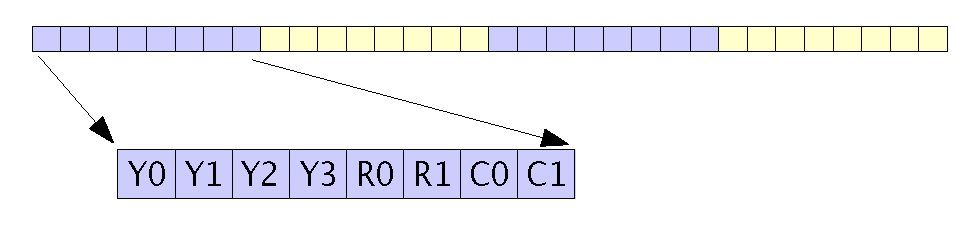
\includegraphics[width=9cm,height=2cm]{sequence.eps}
\caption{Sequence of Product Codes}
\label{sequence}
\end{figure}

\begin{figure}[H]
\center
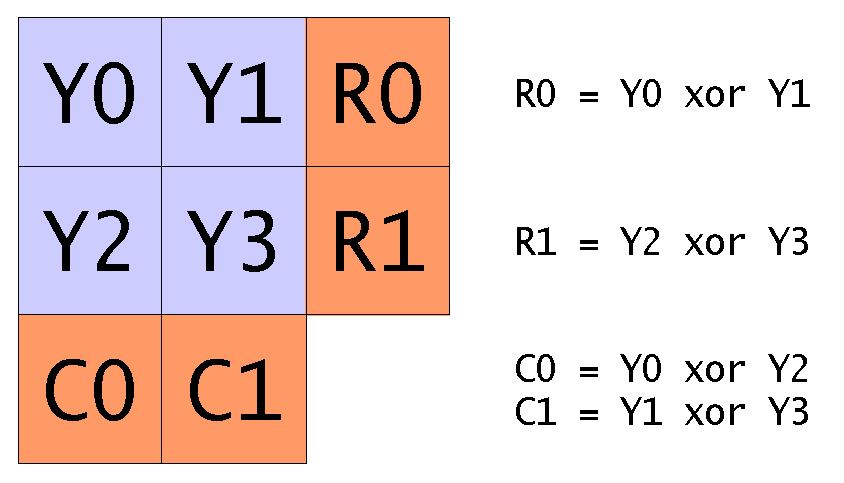
\includegraphics[width=8cm,height=4cm]{product_codes_table.eps}
\caption{Product Code generations}
\label{product_code}
\end{figure}

\section{Decoding Algorithm}

\begin{equation}
posteriori~value = channel~value~(Lch) + priori~value +
external~value~(Le)
\end{equation}

\begin{equation}
\left\{
\begin{array}{lr}
posteriori = Lch~+~priori~+~Le~(row~parity)      & (0)\\
posteriori = Lch~+~priori~+~Le~(column~parity)   & (1)\\
....\\
....\\
posteriori = Lch~+~priori~+~Le~(row~parity)      & (n-1)\\
posteriori = Lch~+~priori~+~Le~(column~parity)   & (n)\\
\end{array}
\right\}
\end{equation}

\begin{equation}
Lch = Y0,~Y1,~Y2,~Y3
\end{equation}

\begin{equation}
priori = posteriori~(n-1)
\end{equation}

\begin{equation}
Le = sgn(a~*~b)~*~min\{abs(a),abs(b)\}
\end{equation}

sgn(a~*~b) means the sign result of multiplication between operand a and
b, and abs(x) means absolute value of operand x. The last value of
posteriori is the decoded informations, i.e the posteriori value at
n$^{th}$ iterations.  The decoded informations can be obtained from the
sign of the last posteriori value, positive value is zero and negative
value is one, i.e this is the most significant bit of the posteriori
value.

\section{Circuit Schematic}

\begin{figure}[H]
\center
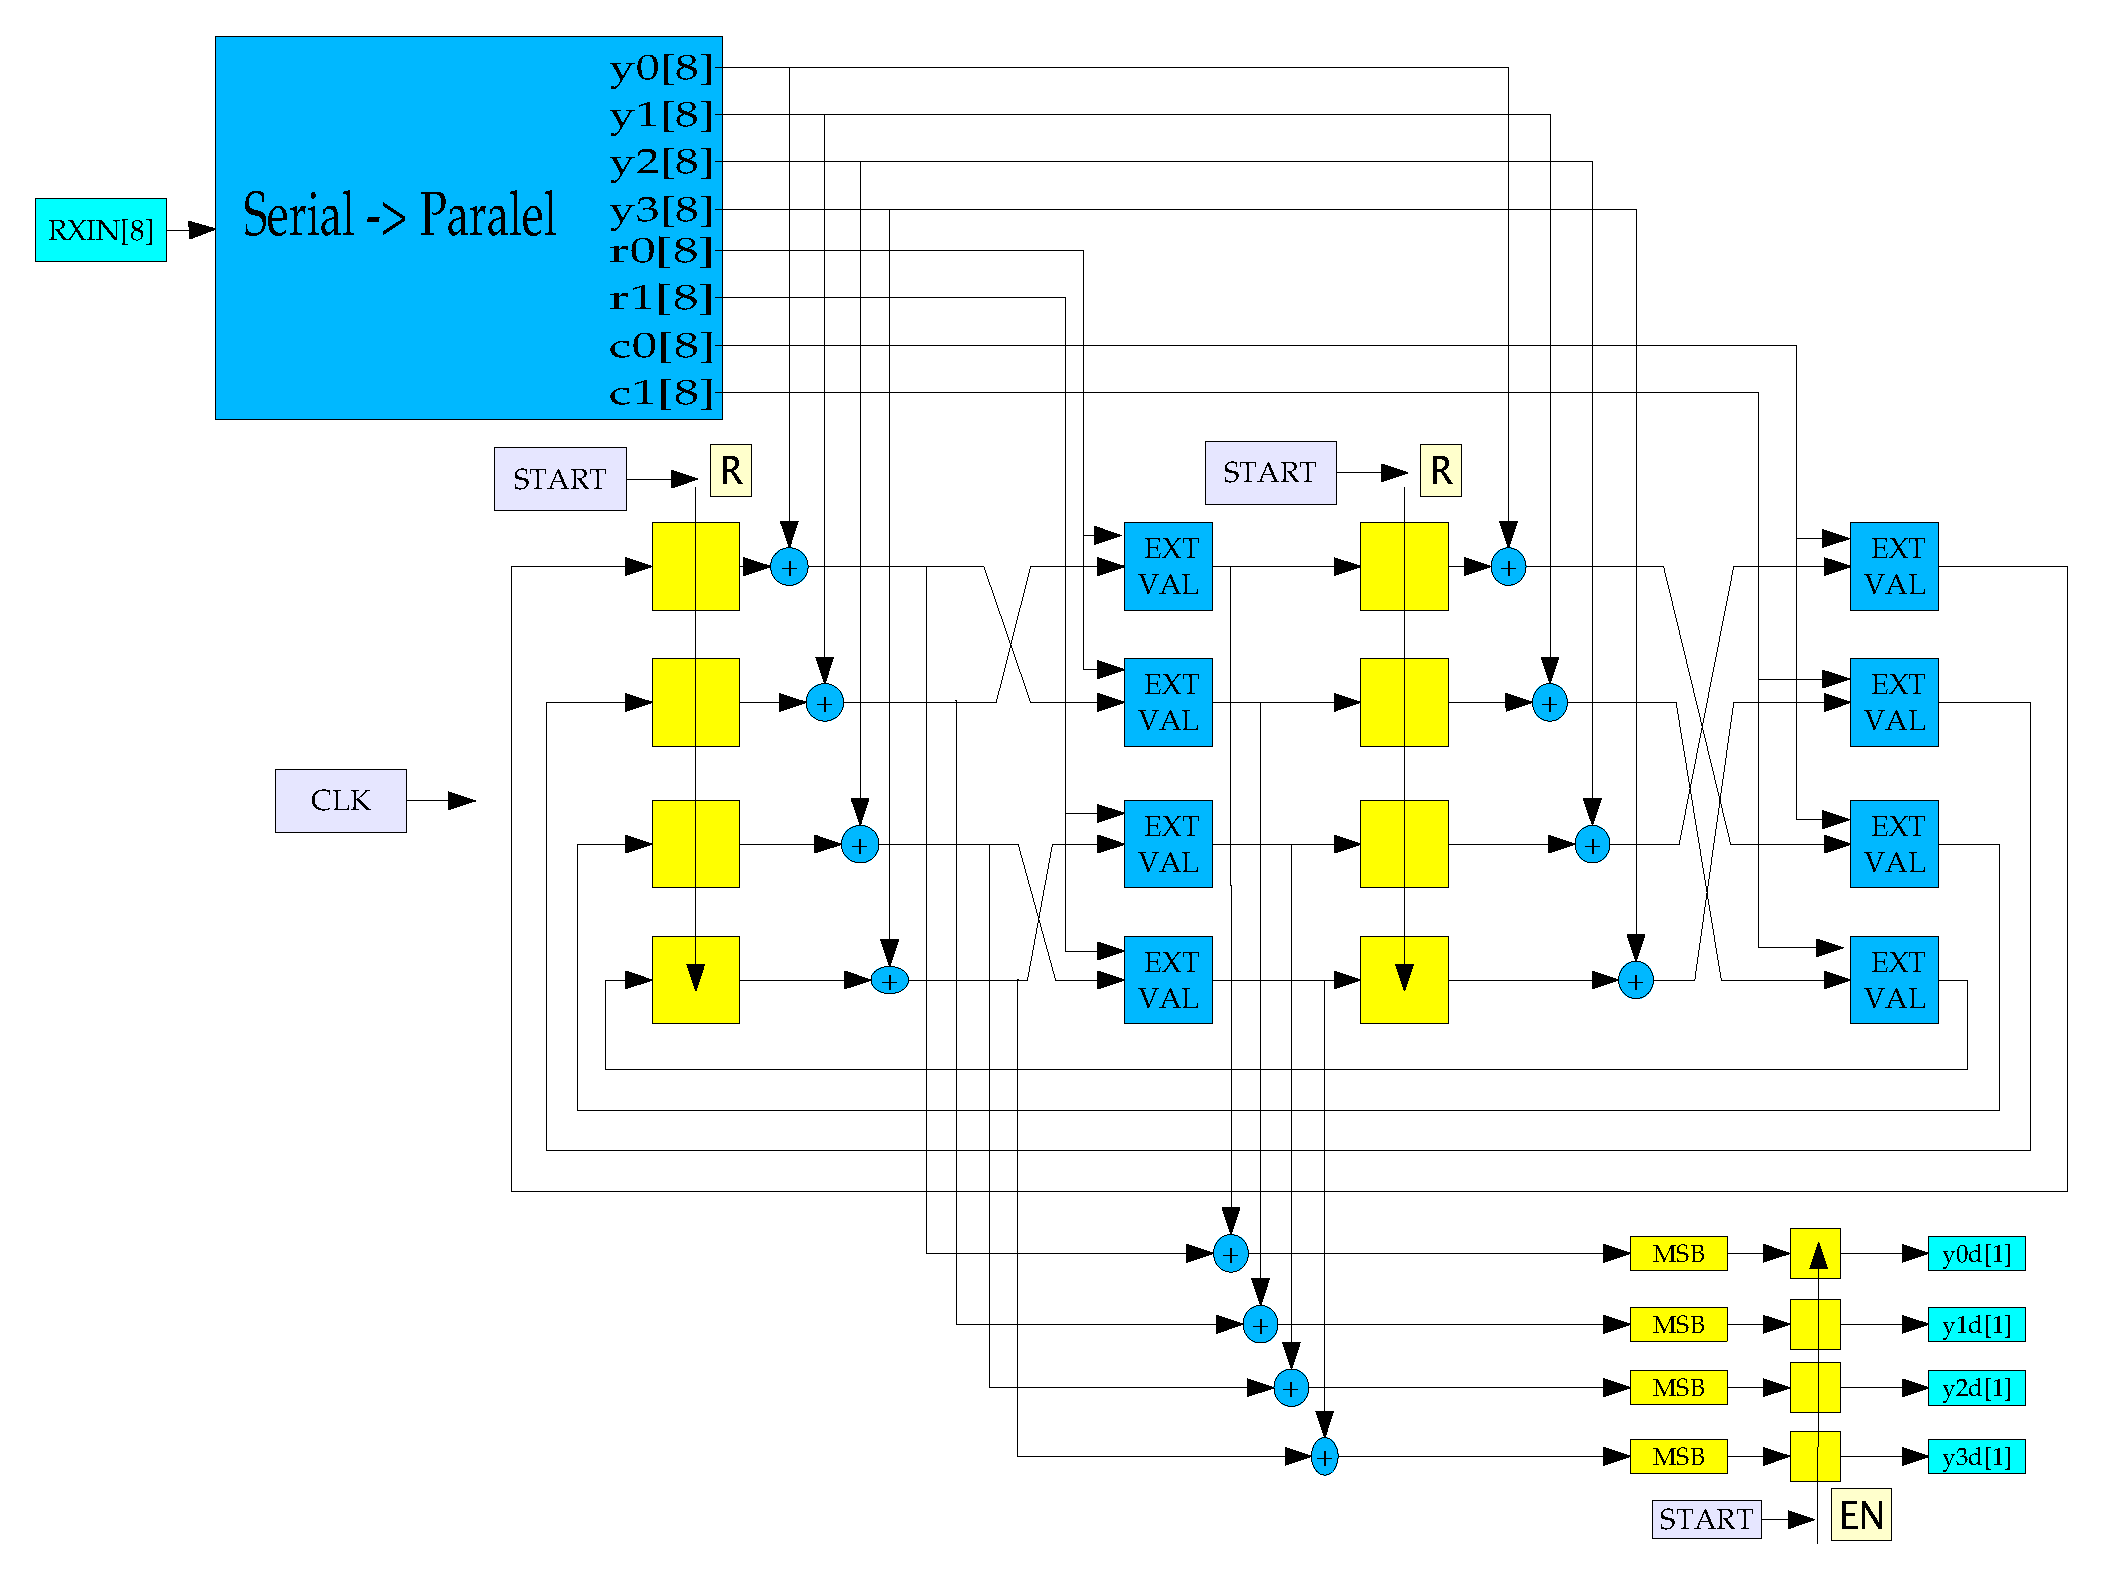
\includegraphics[width=15cm,height=9.0cm]{schematic.eps}
\caption{Schematic of Product Code Decoder}
\label{schematics}
\end{figure}

\chapter{Implementation}

\vspace{2cm}
\section{Simulation}

\begin{figure}[H]
\center
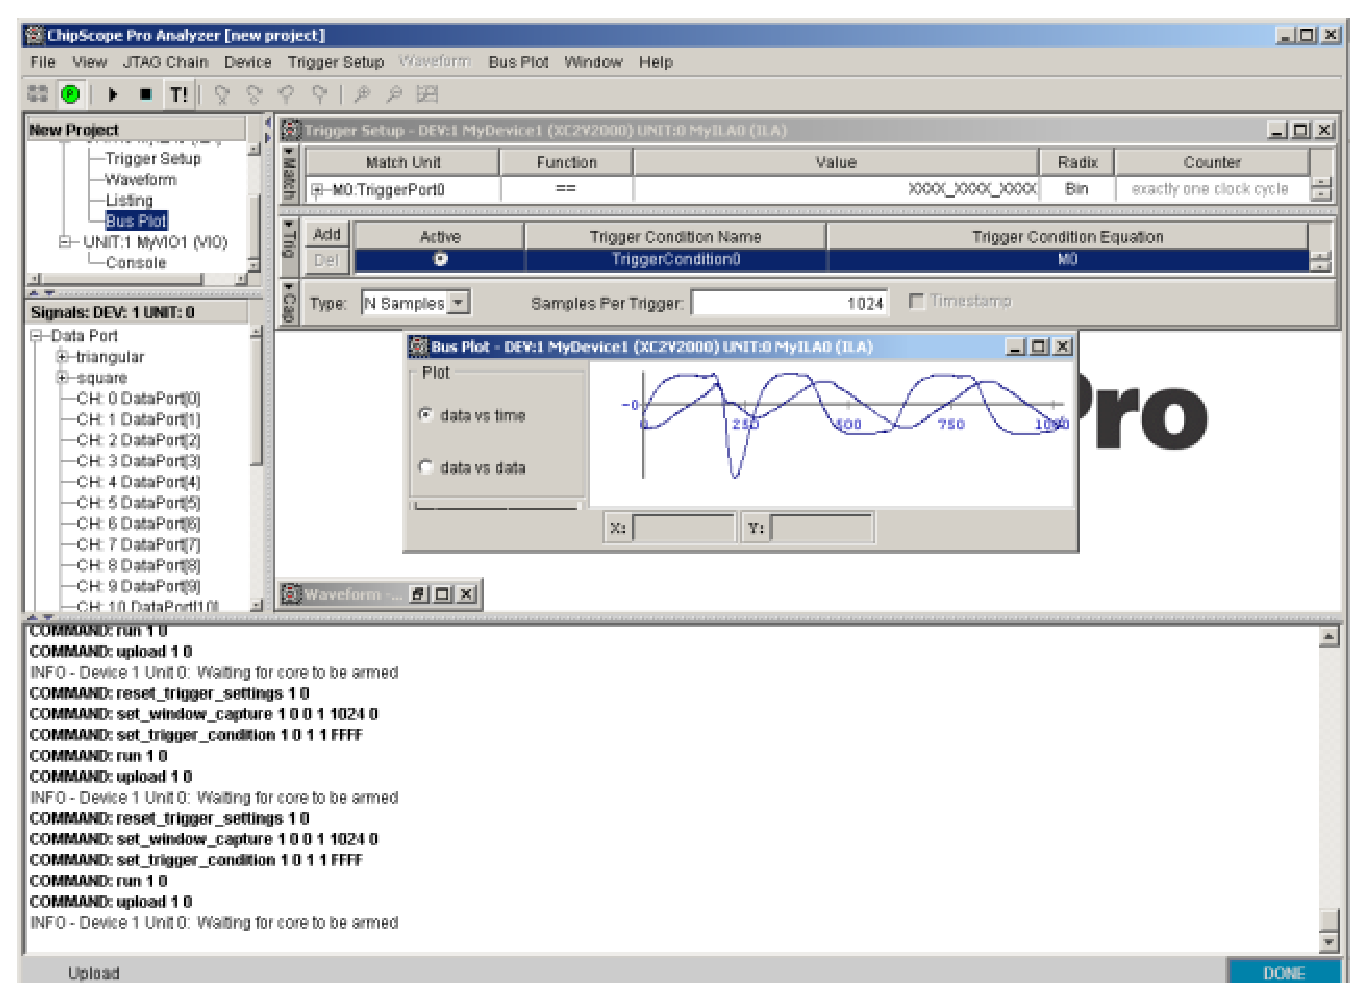
\includegraphics[width=12cm,height=6cm]{screenshot.eps}
\caption{Simulation waveform}
\label{simulation waveform}
\end{figure}

This design has been simulated using ModelSim 6.0 SE, here is the
summary of bit errors on different signal to noise ratio (SNR) of input
signal:

\begin{table}[H]
\center
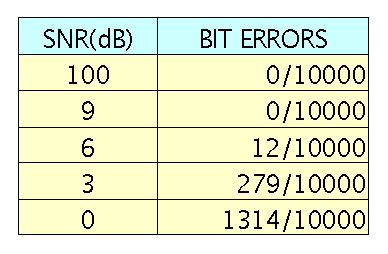
\includegraphics[width=8cm,height=2.5cm]{bit_errors.eps}
\caption{Bit errors on different SNR}
\label{bit_errors}
\end{table}

signal with SNR 0 dB is signal with very big noise.

\section{Synthesize}

This design has been synthesized using ISE Xilinx 6.3i, here is the
summary of the area utilization in FPGA Xilinx:

\begin{table}[H]
\center
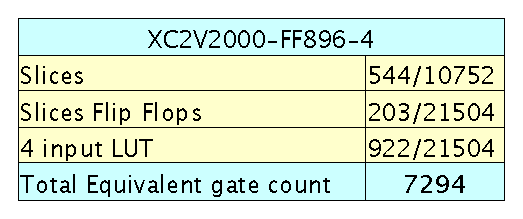
\includegraphics[width=8cm,height=2.5cm]{area.eps}
\caption{Area utilizations summary}
\label{area}
\end{table}

The maximum clock frequency is 64.045 MHz (Minimum period 15.614ns)

\begin{thebibliography}{1}

\bibitem{wada}
Tom Wada, \textbf{2-D Product Code Iterative Decoder},\\
\href{http://www.ie.u-ryukyu.ac.jp/\~\ wada/design06/spec\_e.html}
     {http://www.ie.u-ryukyu.ac.jp/\~\ wada/design06/spec\_e.html}\\
     October 1$^{st}$, 2005

\end{thebibliography}

\appendix

\chapter{Informations}

\section{Warranty}

\begin{center}
\textbf{\texttt{NO WARRANTY}}\\
\end{center}

\textbf{\scriptsize{
THIS SOFTWARE IS PROVIDED BY THE AUTHOR ``AS IS'' AND ANY EXPRESS OR
IMPLIED WARRANTIES, INCLUDING, BUT NOT LIMITED TO, THE IMPLIED WARRANTIES
OF MERCHANTABILITY AND FITNESS FOR A PARTICULAR PURPOSE ARE DISCLAIMED.
IN NO EVENT SHALL THE AUTHOR BE LIABLE FOR ANY DIRECT, INDIRECT,
INCIDENTAL, SPECIAL, EXEMPLARY, OR CONSEQUENTIAL DAMAGES (INCLUDING, BUT
NOT LIMITED TO, PROCUREMENT OF SUBSTITUTE GOODS OR SERVICES; LOSS OF USE,
DATA, OR PROFITS; OR BUSINESS INTERRUPTION) HOWEVER CAUSED AND ON ANY
THEORY OF LIABILITY, WHETHER IN CONTRACT, STRICT LIABILITY, OR TORT
(INCLUDING NEGLIGENCE OR OTHERWISE) ARISING IN ANY WAY OUT OF THE USE OF
THIS SOFTWARE, EVEN IF ADVISED OF THE POSSIBILITY OF SUCH DAMAGE.}}

\section{Tools}

\begin{itemize}
\item ALLIANCE CAD SYSTEM developed by ASIM
      team at \copyright LIP6/Universit\'{e} Pierre et
      Marie Curie,
      \href{http://asim.lip6.fr/recherche/alliance}{\textbf{http://asim.lip6.fr/recherche/alliance}}\\
      The primary VHDL Analyser for Synthesize
\item \textbf{ModelSim 6.0} The Simulator
\item \textbf{Xilinx 6.3i} The Synthesizer
\item \textbf{VIM} (Vi IMproved) The Editor
\item \textbf{\LaTeX}~~The Typesetter
\end{itemize}

\vspace{15cm}
\begin{tabbing}
\textbf{Version: 1.0} 
\end{tabbing}

\end{document}
